%% Document class
\documentclass[12pt,preprint]{aastex}
%\documentclass[preprint2]{aastex}
%\documentclass[iop,revtex4]{emulateapj}

%general packages
\usepackage{amsmath}	%for \text{} in math mode
\usepackage{mathrsfs } %for likelihood L
\usepackage{lscape} % landscape environment

%%Figure packages
\usepackage{grffile}	%for dots in filenames

%%Referencinb
\usepackage{hyperref}

%% Custom macros
\newcommand{\vect}[1]{\boldsymbol{#1}} % Uncomment for BOLD vectors.
%\newcommand{\vect}[1]{\vec{#1}} % Uncomment for ARROW vectors.
\newcommand*\diff{\mathop{}\!\mathrm{d}}
\newcommand*\Diff[1]{\mathop{}\!\mathrm{d^#1}}
\newcommand{\pdf}{\ensuremath{pdf}}
\newcommand{\pmodel}{\ensuremath{p_M}}
\newcommand{\MAP}{{\sl MAP}~}
\newcommand{\MAPs}{{\sl MAP}s~}
\newcommand{\RM}{{\sl RoadMapping}~}
 
%% Abbreviations
\shorttitle{Action-based Dynamical Models for the Milky Way}
\shortauthors{Trick et al.}

\begin{document}

%% Title [TO DO: Decide on one of them]
%\title{The {\sc RoadMapping} Code:\\How to deal with "Real World" Issues\\in Action-based Dynamical Modelling the Milky Way\\}
\title{Action-based Milky Way Disk Modelling with \emph{RoadMapping}\\and our imperfect Knowledge of the "Real World"\\}

%% Authors    
\author{W. Trick\altaffilmark{1,2},  J. Bovy\altaffilmark{3,4}, and H.-W. Rix\altaffilmark{1}}
\email{trick@mpia.de}

%% Affiliations
\altaffiltext{1}{Max-Planck-Institut f\"ur Astronomie, K\"onigstuhl 17, D-69117 Heidelberg, Germany}
\altaffiltext{2}{Correspondence should be addressed to trick@mpia.de.}
\altaffiltext{3}{University of Toronto [TO DO: What is Jo's current address???]}
\altaffiltext{4}{Hubble fellow}


%%%-----------------------------------------------------------------------------------------------------------------------------------------------------------------------------
%% Abstract
%\input{docs/abstract_v2.01}
%%-----------------------------------------------------------------------------------------------------------------------------------------------------------------------------
%
%%% Keywords
%\keywords{Galaxy: disk --- Galaxy: fundamental parameters --- Galaxy: kinematics and dynamics --- Galaxy: structure}
%
%%table of contents (remove later [TO DO])
%%\tableofcontents
%
%%-----------------------------------------------------------------------------------------------------------------------------------------------------------------------------
%%Introduction
%\input{docs/introduction_v2.01}
%%-----------------------------------------------------------------------------------------------------------------------------------------------------------------------------
%
%%-----------------------------------------------------------------------------------------------------------------------------------------------------------------------------
%%Dynamical Modelling
%\input{docs/dynamical_modelling_model_v2.01}
%\input{docs/dynamical_modelling_mockdata_v2.01}
%\subsection{Likelihood} \label{sec:likelihood}

\paragraph{Form of the likelihood.}  As data we use the positions and velocities of stars coming from a given \MAP and survey selection function $\text{sf}(\vect{x})$,
\begin{eqnarray*}
D  =\{ \vect{x}_i,\vect{v}_i \mid && \text{(star $i$ belonging to same \MAP)}\nonumber\\
&\wedge& (\text{sf}(\vect{x_i}) > 0) \}.
\end{eqnarray*}

The model that we fit to the data is a parametrized potential and a single qDF with a given number of fixed and free parameters,
\begin{eqnarray*}
\pmodel =\{ p_\text{DF} , p_\Phi \},
\end{eqnarray*}
We fit the qDF parameters (see \S\ref{sec:qDF}) with a logarithmically flat prior, i.e. flat priors in
\begin{eqnarray*}
p_\text{DF} := \{&& \ln \left(h_R/8\text{kpc}\right), \\
&& \ln \left(\sigma_{R,0}/220\text{km s$^{-1}$}\right), \ln \left(\sigma_{z,0}/220\text{km s$^{-1}$}\right), \\
&& \ln \left(h_{\sigma,R}/8\text{kpc}\right), \ln \left(h_{\sigma,z}/8\text{kpc}\right)\ \}.
\end{eqnarray*}
The orbit of the $i$-th star in a potential with $p_\Phi$ is labeled by the actions $\vect{J}_i := \vect{J}[\vect{x}_i,\vect{v}_i\mid p_{\Phi}]$ and the qDF evaluated for the $i$-th star is then $\text{qDF}(\vect{J}_i \mid \pmodel) := \text{qDF}(\vect{J}[\vect{x}_i,\vect{v}_i\mid p_{\Phi}] \mid p_\text{DF})$.

The likelihood of the data given the model $\mathscr{L} = (D \mid \pmodel)$ is the product of the probabilities for each star to move in the potential with $p_\Phi$, being within the survey's selection function and it's orbit to be drawn from the qDF with $p_\text{DF}$, i.e. 
\begin{eqnarray}
&&\mathscr{L}(\pmodel \mid D) \nonumber\\
&&\equiv \prod_i^{N} P(\vect{x}_i,\vect{v}_i \mid \pmodel) \nonumber\\
&&= \prod_i^{N} \frac{1}{\left(r_o v_o\right)^3} \cdot \frac{\text{qDF}(\vect{J}_i \mid \pmodel) \cdot \text{sf}(\vect{x}_i)}{\int \Diff 3 x \Diff 3 v \  \text{qDF}(\vect{J} \mid \pmodel) \cdot \text{sf}(\vect{x})}\nonumber\\
&&\propto \prod_i^{N} \frac{1}{\left(r_o v_o\right)^3} \cdot \frac{\text{qDF}(\vect{J}_i \mid \pmodel)}{\int \Diff 3 x \  \rho_\text{DF}(R,|z| \mid \pmodel) \cdot \text{sf}(\vect{x})}, \label{eq:prob}
%\label{eq:likelihood}
\end{eqnarray}
where $N$ is the number of stars in the data set $D$.
In the last step we used Equation (\ref{eq:tracerdensity_general}). The factor $\prod_i\text{sf}(\vect{x}_i)$ is independent of the model parameters, so we  simply evaluate Equation (\ref{eq:prob}) in the likelihood calculation. We find the best set of model parameters by maximising the likelihood. 


\paragraph{A word on units.} We evaluate the likelihood in a scale-free potential within a Galactocentric coordinate system which is defined as $v_\text{circ}(R = 1) = 1$. The circular velocity at the sun's radius, $v_\text{circ}(R_\odot = 8. \text{kpc}) \sim 230 \text{km s$^{-1}$}$, determines the total mass amplitude of the galaxy potential. In the modelling all data and model parameters are re-scaled to spatial units of $r_o := R_\odot$ or velocitiy units of $v_o := v_\text{circ}(R_\odot )$. The prefactor $1/\left(r_o v_o\right)^3$ in Equation (\ref{eq:prob}) makes sure that the likelihood has the correct units to satisfy:
\begin{eqnarray*}
\int P(\vect{x},\vect{v} \mid \pmodel) \Diff 3 x \Diff 3 v \propto 1
\end{eqnarray*} 
Including this prefactor is crucial when $v_\text{circ}(R_\odot )$ is a free fitting parameter.

\paragraph{Numerical accuracy in calculating the likelihood.} The normalisation in Equation (\ref{eq:prob}) is a measure for the total number of tracers inside the survey volume,
\begin{equation}
M_\text{tot} \equiv \int \Diff 3 x \  \rho_\text{DF}(R,|z| \mid p_model) \cdot \text{sf}(\vect{x}).\label{eq:normalisation}
\end{equation}
In the case of an axisymmetric galaxy model and $\text{sf}(\vect{x})=1$ everywhere inside the observed volume (i.e. a complete sample as assumed in most tests in this work), the normalisation is essentially a two-dimensional integral in $R$ and $z$ of the interpolated tracer density $\rho_{DF}$ (see Equation (\ref{eq:tracerdensity}) and surrounding text) over the survey volume times the observation volume's geometric angular contribution at each $(R,z)$. We perform this integral as a Gauss Legendre quadrature of order 40 in each $R$ and $z$ direction.
\\Unfortunately the evaluation of the likelihood for only one set of model parameters is computationally expensive. The computation speed is set by the number of action calculations required, i.e. the number of stars and the numerical accuracy of the integrals in Equation (\ref{eq:tracerdensity}) needed for the normalisation, which requires $N_\text{spatial}^2 \times N_\text{velocity}^3$ action calculations. The accuracy has to be chosen high enough, such that a resulting numerical error 
\begin{eqnarray}
&&\delta_{M_{tot}} \nonumber\\
&&\equiv \frac{M_\text{tot}(N_\text{spatial},N_\text{velocity},N_\text{sigma}) -  M_\text{tot,true} }{M_\text{tot,true}}\label{eq:relerrlikelihood}
\end{eqnarray}
does not dominate the likelihood, i.e.
\begin{eqnarray}
& &\log \mathscr{L}(\pmodel \mid D) \nonumber\\
&& = \sum_i^{N} \log \text{qDF}(\vect{J_i} \mid \pmodel) - 3N \log \left( r_o v_o\right)\nonumber\\
& & -N \log(M_\text{tot,true}) - N \log (1 + \delta_{M_{tot}}),\label{eq:loglikelihood_relerr}
\end{eqnarray}
with
\begin{eqnarray}
N \log (1 + \delta_{M_{tot}}) \lesssim 1.\nonumber
\end{eqnarray}
In other words, this error is only small enough, if it does not affect the comparison of two adjacent models whose likelihoods differ, to be clearly distinguishable, by a factor of 10. Otherwise numerical inaccuracies could lead to systematic biases in the potential and DF fitting. For data sets as large as $N =$ 20,000 stars in one \MAP, which in the age of GAIA could very well be the case [TO DO: Really???], we would need a numerical accuracy of 0.005\% in the normalisation. Figure \ref{fig:norm_accuracy} demonstrates that the numerical accuracy we use in the analysis, $N_\text{spatial}=16$, $N_\text{velocity}=24$ and $N_{sigma}=5$, does satisfy this requirement.

%====================================================================

%FIGURE: accuracy in the likelihood normalisation 

\begin{figure*}
\plotone{figs/normalisation_accuracy_3.eps}
\caption{Relative error of the likelihood normalization in Equation (\ref{eq:relerrlikelihood}) depending on the accuracy of the density calculation in Equation (\ref{eq:tracerdensity}) (and sourrounding text). The different colors represent calculations for different radii of the spherical observation volume around the sun, as indicated in the legend. $N_\text{spatial}$ is the number of regular grid points in each $R$ and $z > 0$ within the observed volume on which the tracer density is evaluated according to Equation (\ref{eq:tracerdensity}). At each $(R,z)$ a Gauss-Legendre integration of order $N_\text{velocity}$ is performed over an integration range of $\pm N_\text{spatial}$ times the dispersion in $v_R$ and $v_z$ and $[0,1.5v_\text{circ}(R_\odot)]$ in $v_T$. To integrate the interpolated density over the observed volume to arrive at the likelihood normalization in Equation (\ref{eq:normalisation}), we perform a 40th-order Gauss-Legendre integration in each $R$ and $z$ direction. We compare the convergence of the normalisation for the "hot" qDF in three potentials, "Iso-Pot", "MW13-Pot" and "KKS-Pot" (see also Test \ref{test:norm_accuracy} in Table \ref{tbl:tests} for all other model details). In each column of plots we keep two of the accuracy parameters fixed (indicated on top), while the third parameter is varied. (Caption continues on next page.)} 
\label{fig:norm_accuracy}
\end{figure*}

\addtocounter{figure}{-1}
\begin{figure} [t!]
  \caption{(Continued.) We calculate the true normalization with high accuracy as $M_\text{tot,true} \approx M_\text{tot}(N_\text{spatial}=20,N_\text{velocity}=56,N_\text{sigma}=7)$. The dashed lines indicate the accuracy used in our analyses: it is better than $0.002\%$ for all three potential types. Only for the smallest volume in the "MW13-Pot" (yellow line) the error is only $\sim 0.005\%$. This could be due to the fact, that, while we have analytical formulas to calculate the actions for the isochrone and the Staeckel potential exactly, we have to resort to an approximate action calculation for the MW-like potential (see \S\ref{sec:potentials}). [TO DO: Try to redo yellow curve in MW. Weird, that it does not depend on $N_{spatial}$.???] [TO DO: fancybox Legend]}
\end{figure}


%====================================================================

\paragraph{Dealing with measurement errors.} 

We assume Gaussian errors in the observable space $\vect{y} \equiv (\tilde{\vect{x}},\tilde{\vect{v}})=(\text{RA},\text{DEC},(m-M),\mu_\text{RA},\mu_\text{DEC},v_\text{los})$,
\begin{eqnarray*}
N[\vect{y}_i,\delta \vect{y}_i](\vect{y}') &=& N[\vect{y}',\delta \vect{y}_i](\vect{y}_i)\\ 
&\equiv&  \prod_k \frac{1}{\sqrt{2\pi(\delta {y}_{i,k})^2}} \exp\left( -\frac{(y_{i,k}-y_k')^2}{2(\delta y_{i,k})^2}\right),
\end{eqnarray*}
where $y_{i,k}$ is the $k$-th coordinate in $\vect{y}_i$ of the $i$-th star. Observed stars follow the (quasi-isothermal) distribution function (DF$(\vect{y}) \equiv$ qDF$(\vect{J}[\vect{y} \mid p_\Phi] \mid p_\text{DF}])$ for short), convolved with the error distribution $N[0,\delta y](\vect{y})$. The selection function sf$(\vect{y})$ acts on the space of (error affected) observables. 
Then the probability of one star coming from potential $p_\Phi$, distribution function $p_\text{DF}$ and being affected by the measurement errors $\delta \vect{y}$ becomes
\begin{eqnarray*}
&&\tilde{P}(\vect{y}_i \mid p_\Phi,p_\text{DF},\delta \vect{y}_i)\\
& \equiv& \frac{\text{sf}(\vect{y}_i) \cdot \int \Diff{6} y' \  \text{DF}(\vect{y}') \cdot N[\vect{y}_i,\delta \vect{y}_i](\vect{y}')}{\int \Diff{6}y  \  \text{DF}(\vect{y})  \cdot  \int \Diff{6} y' \  \text{sf}(\vect{y}')  \cdot N[\vect{y},\delta \vect{y}_i](\vect{y}')}.
\end{eqnarray*}
In the case of errors in distance or position, the evaluation of this is computational expensive - especially if the stars' have heteroscedastic errors $\delta \vect{y}_i$, for which the normalisation would have to be calculated for each star separately. In practice we apply the following approximation:
\begin{eqnarray}
&&\tilde{P}(\vect{y}_i \mid p_\Phi,p_\text{DF},\delta \vect{y}_i) \nonumber\\
&\approx& \frac{ \text{sf}(\vect{x}_i)}{\int \Diff{6}y  \  \text{DF}(\vect{y})  \cdot   \text{sf}(\vect{x})} \cdot \frac{1}{N_\text{error}} \sum_n^{N_\text{error}}  \text{DF}(\vect{x}_i,\vect{v}[\vect{y}'_{i,n}]) \label{eq:errorconv}
\end{eqnarray}
with
\begin{eqnarray}
\vect{y}'_{i,n} \sim N[\vect{y}_i,\delta \vect{y}_i](\vect{y}')\nonumber
\end{eqnarray}
In doing so, we ignore errors in the star's position $\vect{x}_i$ altogether. This simplifies the normalisation drastically and makes it independent of measurement errors, including the velocity errors. Distance errors however are included, but only implicitly in the convolution over the stars' velocity errors in the Galactocentric restframe. We calculate the convolution using Monte Carlo integration with $N_\text{error}$ samples drawn from the full error Gaussian in observable space, $y'_{i,n}$. 

%\input{docs/dynamical_modelling_fitting_v2.01}
%%-----------------------------------------------------------------------------------------------------------------------------------------------------------------------------
%
%%-----------------------------------------------------------------------------------------------------------------------------------------------------------------------------
%%Results
%\section{Results} \label{sec:results}

We are now in a position to explore the questions about the ultimate limitations of action based modelling, posed in the introduction: 
\begin{itemize}
\item Can we still retrieve unbiased  model parameter estimates $p_M$ in the limit of large sample sizes? 
\item What role does the survey volume and geometry play, at given sample size? 
\item What if our knowledge of the sample selection function is imperfect, and potentially biased? 
\item How do the parameter estimates deteriorate if the individual errors on the phase-space coordinates become significant? 
\end{itemize}
But we also consider the more fundamental limitations:
\begin{itemize}
\item What if the observed stars are not extacly drawn from the family of model distribution functions? 
\item What happens to the estimate of the potential and the DF, if the actual potential is not contained in the family of model potentials?
\end{itemize}
We do not explore the breakdown of the assumption that the system is axisymmetric and in steady state. Except of the test suite on measurement errors in \S\ref{sec:results_errors}, we assume that the phase-space errors are negligible.


%=========================================




%\input{docs/results_largeData_v2.01}
%\input{docs/results_surveyVolume_v2.01}
%\subsection{What if our assumptions on the (in-)completeness of the data set are incorrect?} \label{sec:results_incompR}

The selection function of a survey could be described by a spatial survey volume and a completeness function, which determines the fraction of stars observed at a given location within the Galaxy with a given brightness, metallicity etc (see \S\ref{sec:selectionfunction}). The completeness function depends on the characteristics and mode of the survey, can be very complex and is therefore sometimes not perfectly known. We investigate how much an imperfect knowledge of the selection function can affect the recovery of the potential. We model this by creating mock data with varying incompleteness, while assuming constant completeness in the analysis. The mock data comes from a sphere around the sun and an incompleteness function that drops linearly with distance $r$ from the sun (see \textcircled{5}, Example 1, in Table \ref{tbl:tests} and Figure \ref{fig:isoSphFlexIncompR_mockdata}).
\\This could be understood as a model for the important effect of stars being less likely to be observed the further away they are. We demonstrate that the potential recovery with \RM is very robust against somewhat wrong assumptions about the (in-)completeness of the data (see Figure \ref{fig:isoSphFlexIncompR_violins}). A lot of information about the potential comes from the rotation curve measurements in the plane, which is not affected by applying an incompleteness function. In Appendix \S\ref{sec:incompZ} we also show that the robustness is somewhat less striking but still given for small misjudgments of the incompleteness in vertical direction, parallel to the disk plane (Figures \ref{fig:isoSphFlexIncompZ_mockdata} and \ref{fig:isoSphFlexIncompZ_violins}). This could model the effect of wrong corrections for dust obscuration in the plane. We also investigate in Appendix \S\ref{sec:incompZ} if indeed most of the information is stored in the rotation curve. For this we use the same mock data sets as analysed in Figures \ref{fig:isoSphFlexIncompR_violins} and \ref{fig:isoSphFlexIncompZ_violins}, but this time we’re not including the tangential velocities in the modelling, rather marginalizing the likelihood over $v_T$. In this case the potential is much less tightly constrained, even for 20,000 stars. For only small deviations of true and assumed completeness ($\lesssim 10\%$) we can however still incorporate the true potential in our fitting result (see Figure \ref{fig:isoSphFlexIncomp_marginal_violins}). 



%FIGURE: isoSphFlexIncompR in mock data space

\begin{figure}
\includegraphics[width=\columnwidth]{figs/isoSphFlexIncompR_mockdata.eps}
\caption{Selection function and mock data distribution for investigating radial incompleteness of the data. All model parameters are summarized as test \textcircled{5}, Example 1, in Table \ref{tbl:tests}. The survey volume is a sphere around the sun and the percentage of observed stars is decreasing linearly with radius from the sun, as demonstrated in the left panel. How fast this detection/incompleteness rate drops is quantified by the factor $\epsilon_r$. Histograms for four data sets, drawn from two \MAPs ("hot" in red and "cool" in blue, see Table \ref{tbl:referenceMAPs}) and with two different $\epsilon_r$, 0 and 0.7, are shown in the right panel for illustration purposes.} 
\label{fig:isoSphFlexIncompR_mockdata}
\end{figure}

%FIGURE: isoSphFlexIncompR

\begin{figure*}
\centering
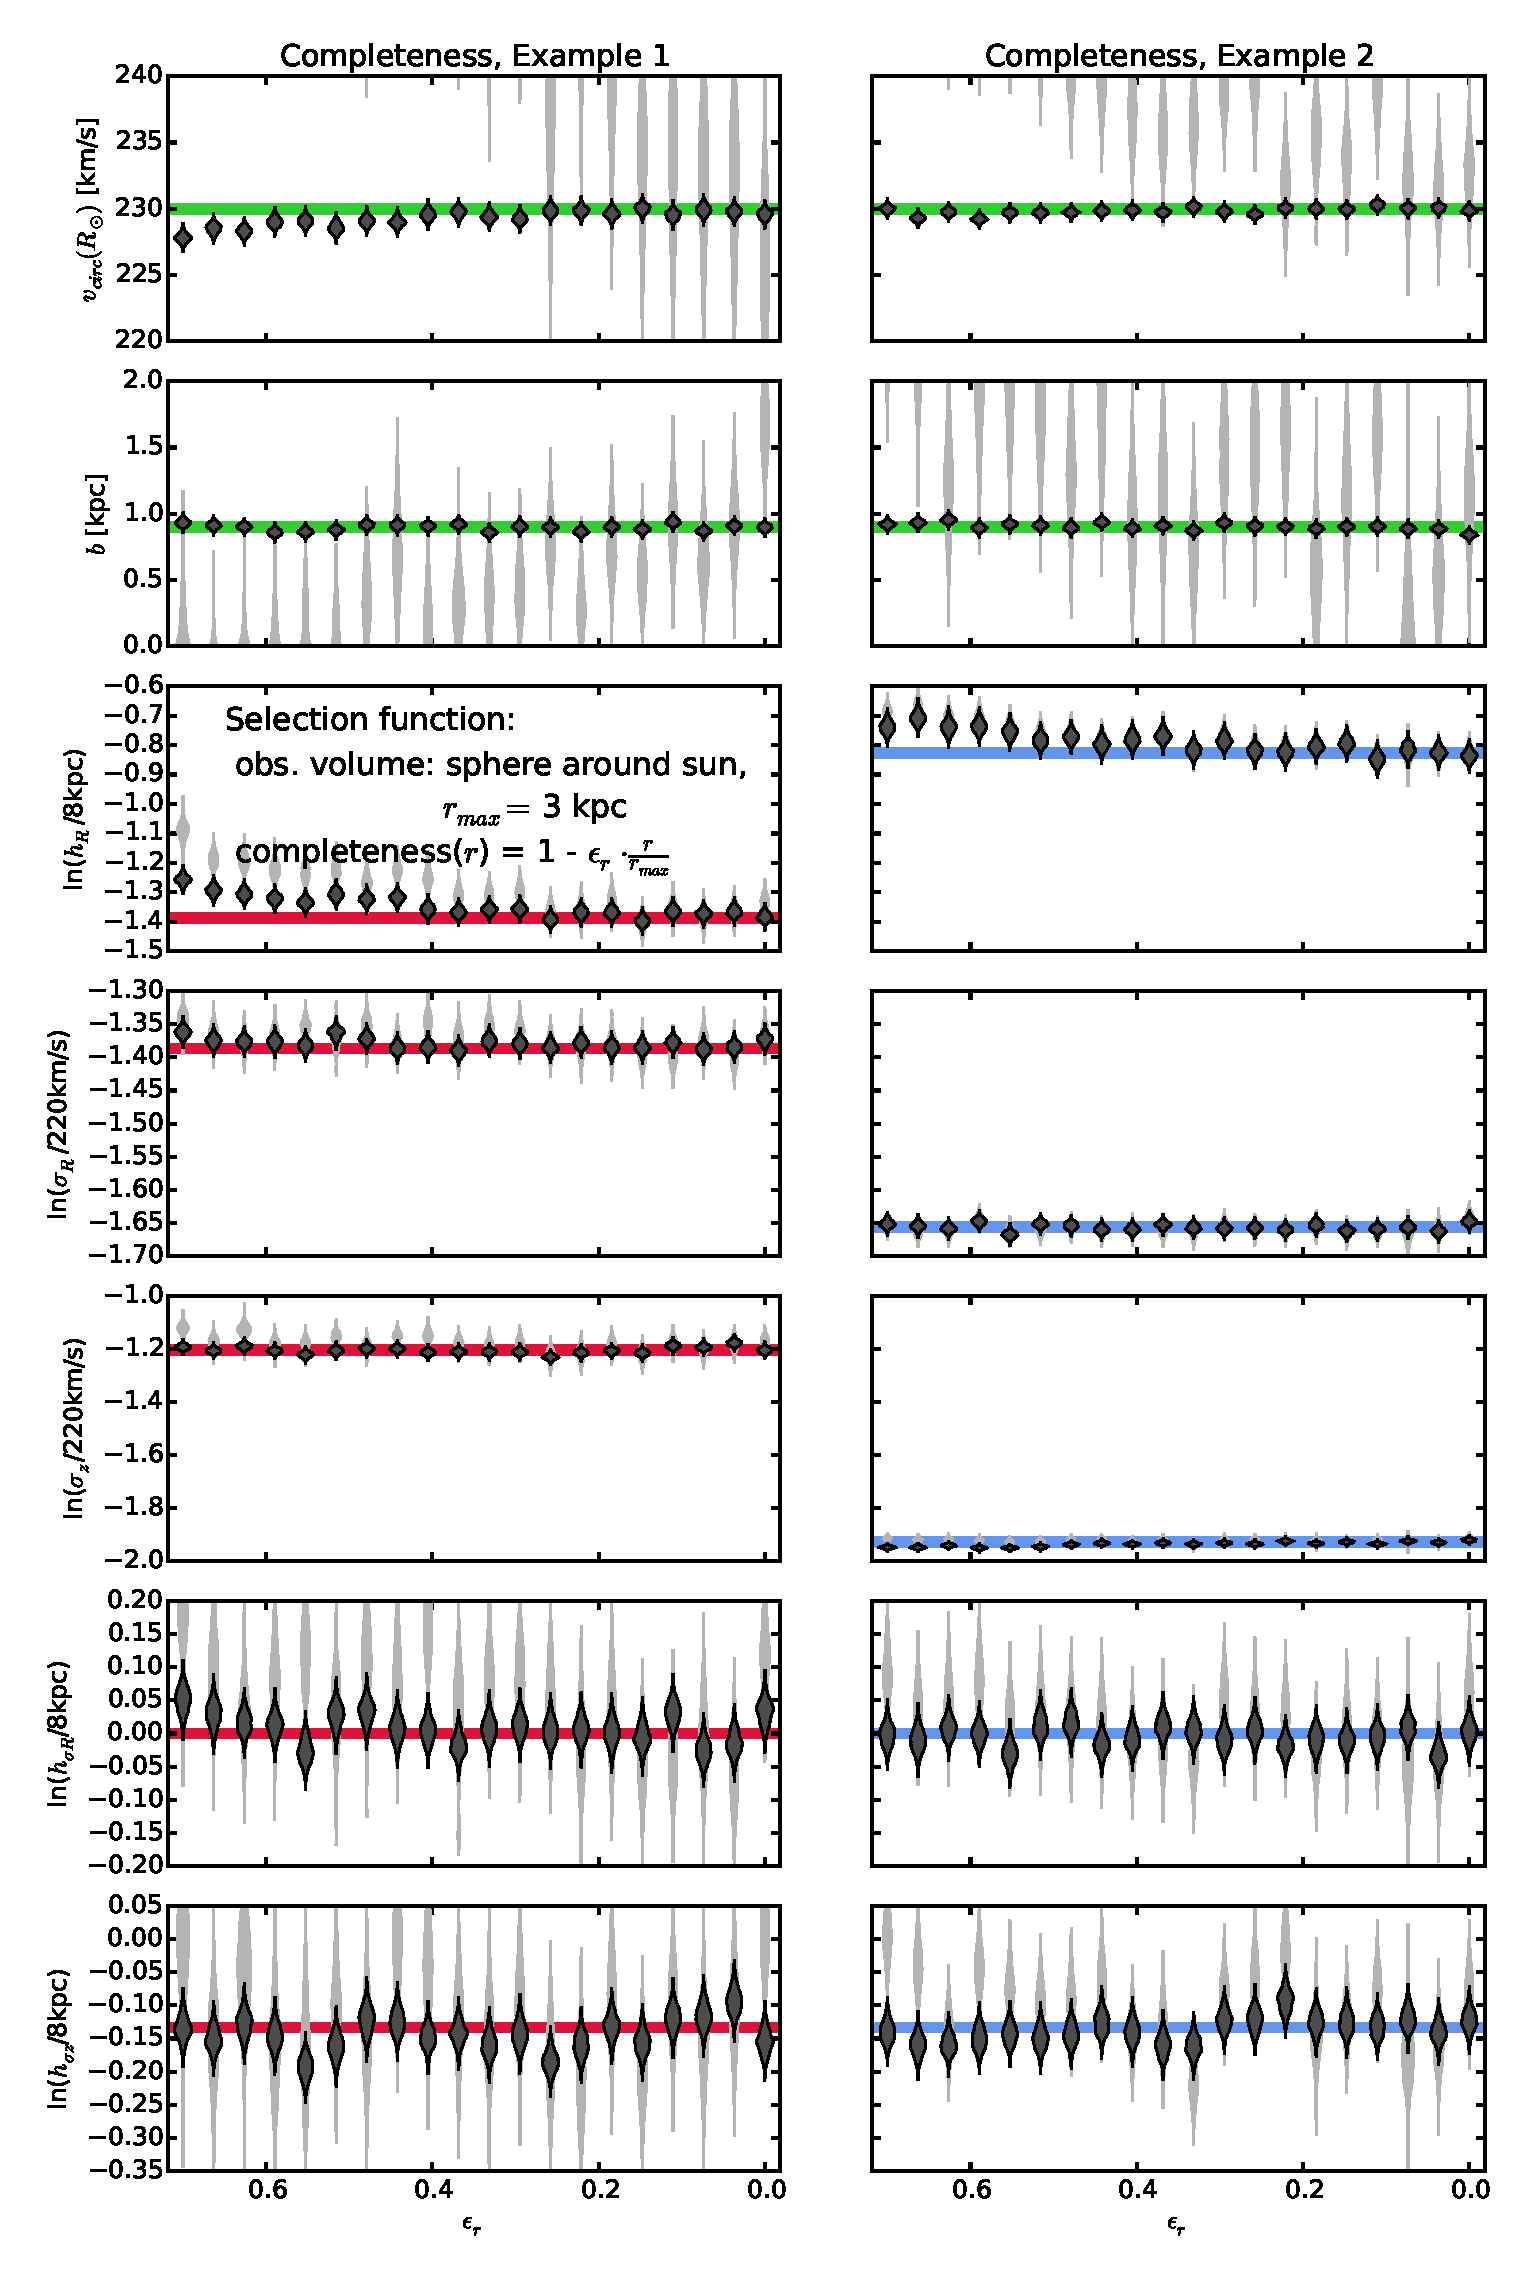
\includegraphics[width=0.8\textwidth]{figs/isoSphFlexIncompR_violins.eps}
\caption{(Caption on next page.)}
\end{figure*}


\addtocounter{figure}{-1}
\begin{figure*} [t!]
\caption{Influence of wrong assumptions about the radial incompleteness of the data on the parameter recovery with \RM. Each mock data set was created having different incompleteness parameters $\epsilon_r$ (shown on the $x$-axis and illustrated in Figure \ref{fig:isoSphFlexIncompR_mockdata}) and the model parameters are given as test \textcircled{5}, Example 1, in Table \ref{tbl:tests}. The analysis however didn't know about the incompleteness and assumed that all data sets had constant completeness within the survey volume ($\epsilon_r = 0$). The marginalized likelihoods from the fits are shown as violins. The green lines mark the true potential parameters ("Iso-Pot") and the red and blue lines the true qDF parameters ("hot" \MAP in red and "cool" \MAP in blue), which we tried to recover. The \RM method seems to be very robust against small to intermediate deviations between the true and the assumed data incompleteness.} 
\label{fig:isoSphFlexIncompR_violins}
\end{figure*}


\subsection{Effect of measurement errors on recovery of potential?} \label{sec:results_errors}

[TO DO]

\paragraph{Collection tests and plots (tests are still running on the cluster)}

\begin{itemize}
\item \emph{Plot 1:} number of MC samples needed for the error convolution vs. maximum velocity error inside the observed volume, such that a given accuracy in potential and qDF parameters is reached. Similar to what I had on the poster. However, we still haven't tested, if this plot depends on: hotness of stars and or umber of stars.

\item \emph{Plot 2:} 2 columns of panels (one row for each parameter), bias vs. standard error. First column: only proper motion and vlos errors $\longrightarrow$ shows that our error convolution works and should be bias free, plus, when knowing the errors perfectly we can get a perfect deconvolution and tight constraints. Second column: proper motion, vlos and distance modulus errors $\longrightarrow$ shows that for too large proper motion and distance errors our approximation for the error convolution does not work anymore.

\end{itemize}

\paragraph{Convergence of the error integral.} In \S \ref{sec:likelihood} we introduced how we convolve the model probability with the measurement errors. In the absence of distance errors the accuracy of the parameter recovery is limited by an insufficient MC sampling of the convolution integral in Eq. (\ref{errorconv}). Test \textcircled{6} in Table \ref{tbl:tests} and Fig. \ref{fig:isoSphFlexErrConv_MC_vs_error} investigate how many MC samples are needed, given the size of the velocity error, for the integral to be accurate within certain limits:
\\For each $\delta \mu \in [2,3,4,5] \text{mas yr}^{-1}$ we set up four mock data sets and evaluated the likelihood for different $N_\text{error}$. We used $N_\text{conv} :=$ 800 and 1200 MC samples to calculate the numerically converged likelihood for proper motion errors $\delta \mu \leq 3 \text{mas yr}^{-1}$ and $\delta \mu > 3 \text{mas yr}^{-1}$, respectively. We determined the mean bias 
\begin{equation*}
\text{BIAS}(N_\text{error},\delta \mu) \equiv \frac{1}{4} \sum_{j=1}^4 \left[ \langle p_i \rangle (N_\text{error},\delta \mu)\right]_j - \left[ \langle p_i \rangle (N_\text{conv},\delta \mu)\right]_j,
\end{equation*}
where $\left[ \langle p_i \rangle (N_\text{error},\delta \mu)\right]_j$ is the best estimate for the $i$-th model parameter $p_i \in \pmodel$ from the analysis of the $j$-th mock data realisation with $\delta \mu$ using $N_\text{error}$ MC samples. From this we then generated the curves $N_{\text{error},i} (\delta v_\text{max},\text{BIAS})$ in Fig. \ref{fig:isoSphFlexErrConv_MC_vs_error} by linear interplolation, that show how many MC samples are needed for parameter $p_i$ given a velocity error and a systematic bias in units of the standard error (SE) of the estimate. The proper motion error $\delta \mu$ translates to a velocity error according to 
\begin{equation}
\delta v_\text{max} [\text{km s}^{-1}] \equiv 4.74047 \cdot r_\text{max}[\text{kpc}] \cdot \delta \mu [\text{mas yr}^{-1}], \label{eq:vmax}
\end{equation}
where $r_\text{max}$ is the maximum distance of stars. We find in Fig. \ref{fig:isoSphFlexErrConv_MC_vs_error} the relation
\begin{equation*}
N_{\text{error},i} (\delta v_\text{max},\text{BIAS}) \propto \left( \delta v_\text{max} \right)^2.
\end{equation*}
Fig. \ref{fig:isoSphFlexErrConv_MC_vs_error} also demonstrates that different model parameters do not have the same sensitivity to the numerical inaccuracies introduced by insufficient sampling. 



\paragraph{Underestimation of the proper motion error.} We found that in case we perfectly knew the measurement errors (and the distance error is negligible), the convolution of the model probability with the measurement errors gives precise and accurate constraints on the model parameters - even if the error itself is quite large. Now we investigate what would happen if the quoted measurement errors, e.g. the proper motion errors, were actually smaller than the true errors. Figure \ref{fig:isoSphFlexErrSyst} shows the case for two different stellar populations and an error underestimation of 10\% and 50\%. 
\\Overall the parameter recovery gets worse the larger the proper motion error and the stronger the underestimation. The relation between the bias due to error misjudgment and the size of the proper motion error seems to be linear.
\\For the recovery of the isochrone potential scale length $b$ the hotness of the population does not matter (see lower left panel in Figure \ref{fig:isoSphFlexErrSyst}). The circular velocity $v_\text{circ}(R_\odot)$ is, as always, better measured by cooler than by hotter populations (see upper left panel in Figure \ref{fig:isoSphFlexErrSyst}). 
\\We find that the recovery of the qDF parameters on the other hand is more strongly affected by the misjudgment of the velocity error for \emph{cooler} stellar popluations. The measured velocity dispersion is the convolution of the intrinsic dispersion with the measurement errors. If the proper motion error is underestimated, the deconvolved velocity dispersion is larger than the intrinsic velocity dispersion and the relative difference is bigger for a cooler population (see upper right panel for $\sigma_z$ in Figure \ref{fig:isoSphFlexErrSyst}). The intrinsic velocity dispersion is also cooler at larger radii than at smaller radii, therefore the deconvolved dispersion is overestimated more strongly at large $R$ and the velocity dispersion scale length will be overestimated as well (see lower left panel for $h_{\sigma_z}$ in Figure \ref{fig:isoSphFlexErrSyst}). We get analogous results for the qDF parameters $\sigma_R$ and $h_{\sigma_R}$. The recovery of the tracer density scale length $h_R$ is not affected by the misjudgment of velocity errors. 
\\The most important and encouraging result from Figure \ref{fig:isoSphFlexErrSyst} is, that for an underestimation of $10\%$ the bias is still $\lesssim 2 \sigma$ - even for proper motion errors of $3$ mas/yr.

%=============================================================

\begin{figure*}
\plotone{figs/isoSphFlexErrConv_MC_vs_error.eps}
\caption{Number of Monte Carlo (MC) samples $N_\text{error}$ needed for the numerical error convolution in Eq. (\ref{eq:errorconv}), given the maximum velocity error $\delta v_\text{max}$ in the sample to reach a given accuracy.  An insufficient sampling of the convolution integral leads to systematic biases in the reconstruction of the true model parameters. The size of the bias is color coded as indicated in the legend and is given in units of the standard error (SE).  The model parameters, marked by different symbols, have different sensitivities to the numerical inaccuracy of the error convolution, therefore the range in $N_\text{error}$ for the same given bias. Here we assume that the distance error is zero and the proper motion error $\delta \mu$ translates to a velocity error according to Eq. (\ref{eq:vmax}) and $\delta v_\text{los} \ll \delta v_\text{max}$. All model parameters are listed in Table \ref{tbl:tests} as Test \textcircled{6}. The number of MC samples needed increases with the velocity error as $N_\text{error} \propto \left( \delta v_\text{max} \right)^2$, as can be seen especially well in the inset figure for the potential parameter $v_\text{circ}(R_\odot)$. All lines are fits of this functional form to each four points derived for a given model parameter (symbol) and bias (color). The large scatter in the points comes from low number statistics and errors introduced by linear interpolation of the bias vs. $N_\text{error}$ relation found from the analyses.}
\label{fig:isoSphFlexErrConv_MC_vs_error}
\end{figure*}


%=============================================================

\begin{figure*}
\plotone{figs/isoSphFlexErrConv_bias_vs_SE.eps}
\caption{[TO DO: Caption]}
\label{fig:isoSphFlexErrConv_bias_vs_SE}
\end{figure*}




%=============================================================

\begin{figure*}
\plotone{figs/isoSphFlexErrSyst_offset_vs_error.eps}
\caption{Effect of an systematic underestimation of proper motion errors in the recovery of the model parameters. The true model parameters used to create the mock data are summarized as Test \textcircled{11} in Table \ref{tbl:tests}, four of them are given on the $y$-axes and the true values are indicated as black dashed lines. The velocities of the mock data were perturbed according to Gaussian errors in the $\alpha$ and $\delta$ proper motions as indicated on the $x$-axis.   The circles and triangles are the best fit parameters of several mock data set assuming the proper motion error, with which the model probability was convolved, was underestimated in the analysis by 10\% or 50\%, respectively. The error bars correspond to $1\sigma$ confidence. The lines connect the mean of each two data realisations and are just guides to the eyes.}
\label{fig:isoSphFlexErrSyst}
\end{figure*}

%=============================================================
%\subsection{The Impact of Deviations of the Data from the Idealized qDF} \label{sec:results_mixedDFs}

%Motivation of the test and what we're doing
Our modelling approach assumes that each \MAP follows a quasi-isothermal distribution function, qDF. In this Section we explore what happens if this idealization does not hold. This could be, because even in the limit of perfectly measured abundances, \MAPs do not follow a qDF. Or, even if they do follow a qDF, the finite abundance errors effectively mix different \MAPs. We investigate both these issues by creating mock data sets (Figure \ref{fig:isoSphFlexMix_mockdata_residuals}) that are drawn from two distinct qDFs of different temperature, and analyze the composite mock data set by fitting a single qDF to it. These results are illustrated in Figs. \ref{fig:isoSphFlexMixCont} and \ref{fig:isoSphFlexMixDiff}. Following the observational evidence, \MAPs with cooler qDFs also have longer tracer scale lengths. In the first set of test, we choose qDFs of widely different temperatures and vary their relative fraction (dubbed ``Examples 1a/b" in Figure \ref{fig:isoSphFlexMixCont} and Test \textcircled{7} in Table \ref{tbl:tests}); in the second set of tests (``Examples 2a/b" in Figure \ref{fig:isoSphFlexMixDiff} and Test \textcircled{7} in Table \ref{tbl:tests}), we always mix mock data points from two different qDFs in equal proportion, but vary by how much the qDF's temperatures differ. 
\\The first set of tests mimics a DF that has wider wings or a sharper core in velocity space than a qDF (Figure \ref{fig:isoSphFlexMix_mockdata_residuals}). The second test could be understood as mixing neighbouring \MAPs due to too large bin sizes or abundance measurement errors.

%What we see in the plot
It is worth considering separately the impact of the DF deviations on the recovery of the potential and of the qDF parameters. 
\\We find from Example 1 that the potential parameters can be better and more robustly recovered, if a mock-data \MAP is polluted by a modest fraction ($\lesssim 30\%$) of stars drawn from a much cooler qDF with a longer scale length, as opposed to the same pollution of stars drawn from a hotter qDF with a shorter scale length. 
\\When considering the case of a 50/50 mix of contributions from different qDFs in Example 2, there is a systematic, but only small, error in recovering the potential parameters, monotonically increasing with the qDF parameter difference; in particular for fractional differences in the qDF parameters of $\lesssim 20\%$ the systematics are insignificant even for samples sizes of 20,000, as used in the mock data. 
\\Overall, a cooler DF seems to always give tighter constraints on the circular velocity at the sun $v_\text{circ}(R_\odot)$, because the rotation curve can be constrained easier if more stars are on near-circular orbits. But the recovered $v_\text{circ}(R_\odot)$ does not necessarily have to be right. The hotter DFs give less tight constraints and are therefore more forgiving.
\\The recovery of the effective qDF parameters, in light of non-qDF mock data is quite intuitive: the effective qDF temperature lies between the two temperatures from which the mixed DF of the mock data was drawn; in all cases the scale length of the velocity dispersion fall-off, $h_{\sigma R}$ and $h_{\sigma , z}$, is shorter, because the stars drawn form the hotter qDF dominate at small radii, while stars form the cooler qDF (with its longer tracer scale length) dominate at large radii. The recovered tracer scale lengths, $h_R$ vary smoothly between the input values of the two qDFs that entered the mix of mock data, with again the impact of contamination by a hotter qDF (with its shorter scale length in this case) being more important. 



%====================================================================

%FIGURE: isoSphFlexMix_mockdata_residuals

\begin{figure*}
\plotone{figs/isoSphFlexMix_mockdata_residuals.eps}
\caption{Distribution of mock data, created by mixing stars drawn from two different qDFs (solid lines), and the distribution predicted by the best fit of a single qDF and potential to the data (dashed lines). The model parameters to create the mock data (solid lines) are given in Table \ref{tbl:tests} as Test \textcircled{7}, and the qDF parameters referenced in the figure's legend are given in Table \ref{tbl:referenceMAPs}. The corresponding single qDF best fit curves (dashed lines) were created by drawing mock data from the best fit parameters found in Figures \ref{fig:isoSphFlexMixCont} and \ref{fig:isoSphFlexMixDiff}. \emph{Example 1:} Distribution of mock data drawn from a superposition of two very different (but fixed) qDFs at varying mixing rates. \emph{Example 2:} Mock data distribution of two \MAPs that were mixed at a fixed rate of 50\%/50\%, but the difference of the qDF parameters of one \MAP was varied with respect to the qDF parameters of the other \MAP by $X\%$ (see Table \ref{tbl:referenceMAPs}). The data sets are color coded in the same way as the corresponding analyses in Figures  \ref{fig:isoSphFlexMixCont} and \ref{fig:isoSphFlexMixDiff}. This figure demonstrates how mixing two qDFs can be used as a test case for changing the shape of the DF to not follow a pure qDF anymore, e.g. by adding wings or slightly changing the radial density profile. When comparing the mock data and best fit distribution, we see that especially for the most extreme deviations it becomes obvious that a single qDF is a bad assumption for the stars' "true" DF.}
\label{fig:isoSphFlexMix_mockdata_residuals}
\end{figure*}


%FIGURE: isoSphFlexMixCont

\begin{figure*}
\centering
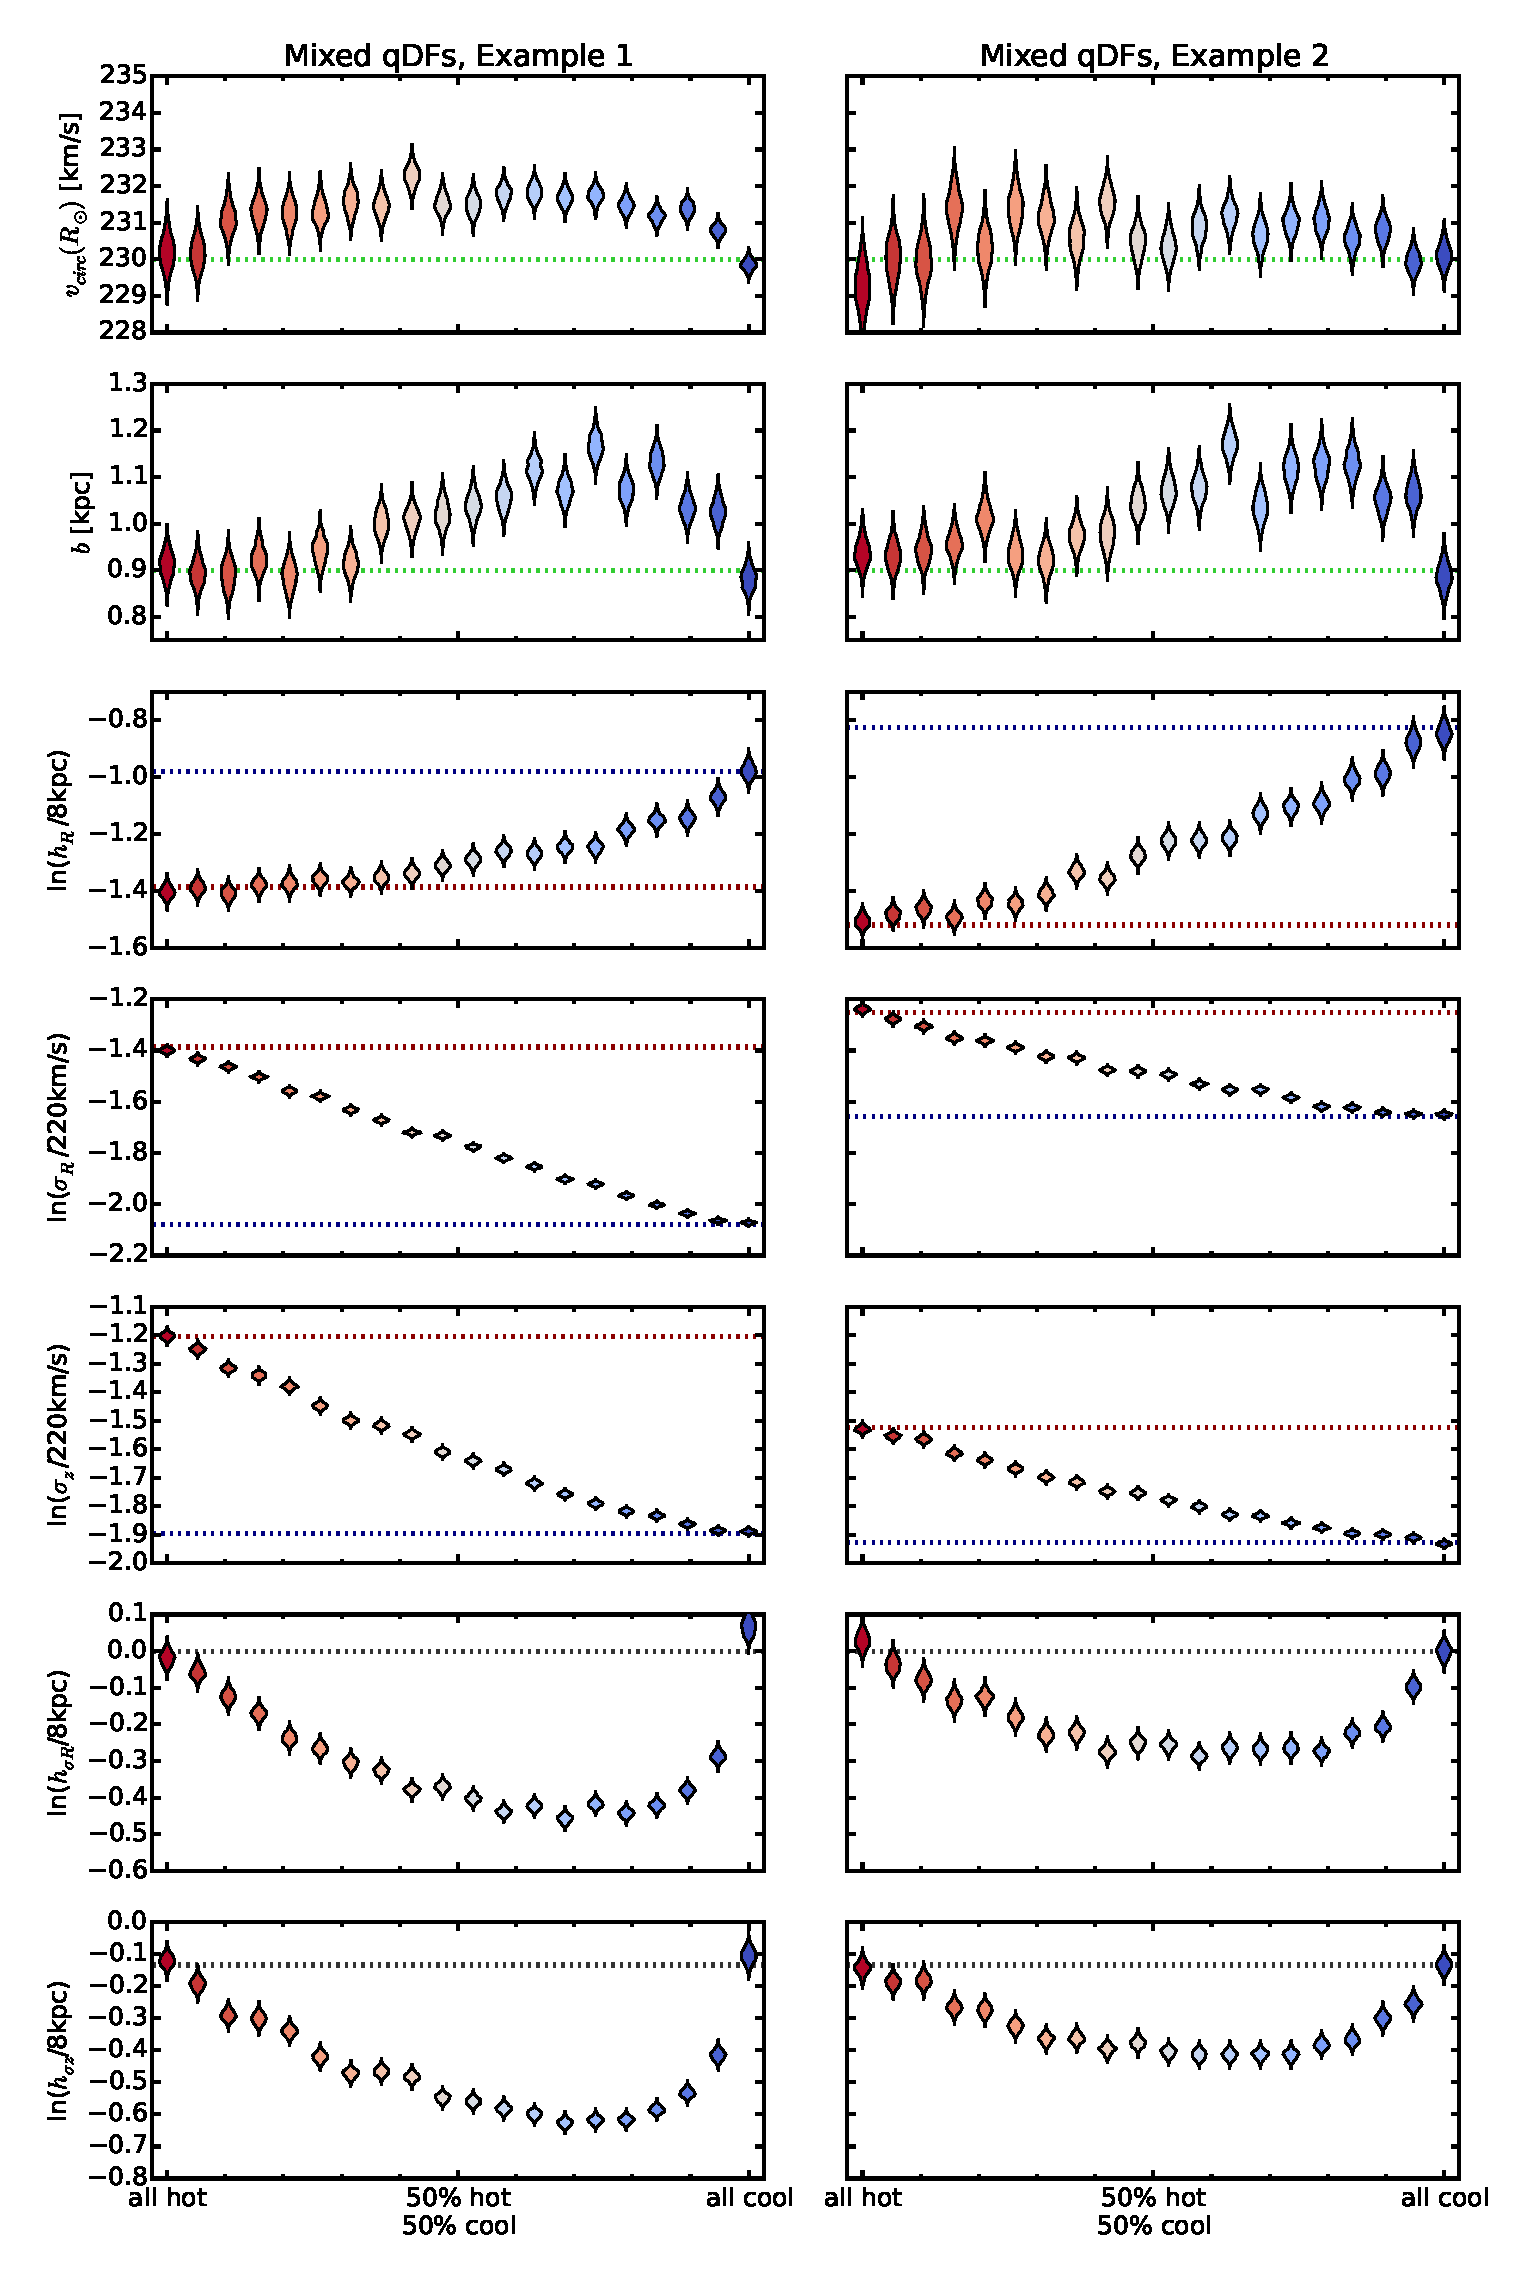
\includegraphics[width=0.8\textwidth]{figs/isoSphFlexMixCont_violins.eps}
\caption{(Caption on next page.)}
\end{figure*}


\addtocounter{figure}{-1}
\begin{figure*} [t!]
\caption{The dependence of the parameter recovery on degree of pollution and temperature of the stellar population. To model the pollution of a hot stellar population by stars coming from a cool population and vice versa, we mix varying amounts of stars from two very different populations, as indicated on the $X$-axis. The composite mock data set is then fit with one single qDF. The violins represent the marginalized likelihoods found from the MCMC analysis. \emph{Example 1a} (\emph{Example 1b}) in the left (right) panels mixes the "hot" ("cool") \MAP with the "cooler" ("hotter") \MAP in Table \ref{tbl:referenceMAPs}. All model parameters used to create the mock data are given in Test \textcircled{7}, \emph{Example 1a) \& b)} in Table \ref{tbl:tests}. Some mock data sets are shown in Figure \ref{fig:isoSphFlexMix_mockdata_residuals}, first two rows, in the same colors as the violins here.  We find, that a hot population is much less affected by pollution with stars from a cooler population than vice versa.}
\label{fig:isoSphFlexMixCont}
\end{figure*}



%FIGURE: isoSphFlexMixDiff

\begin{figure*}
\centering
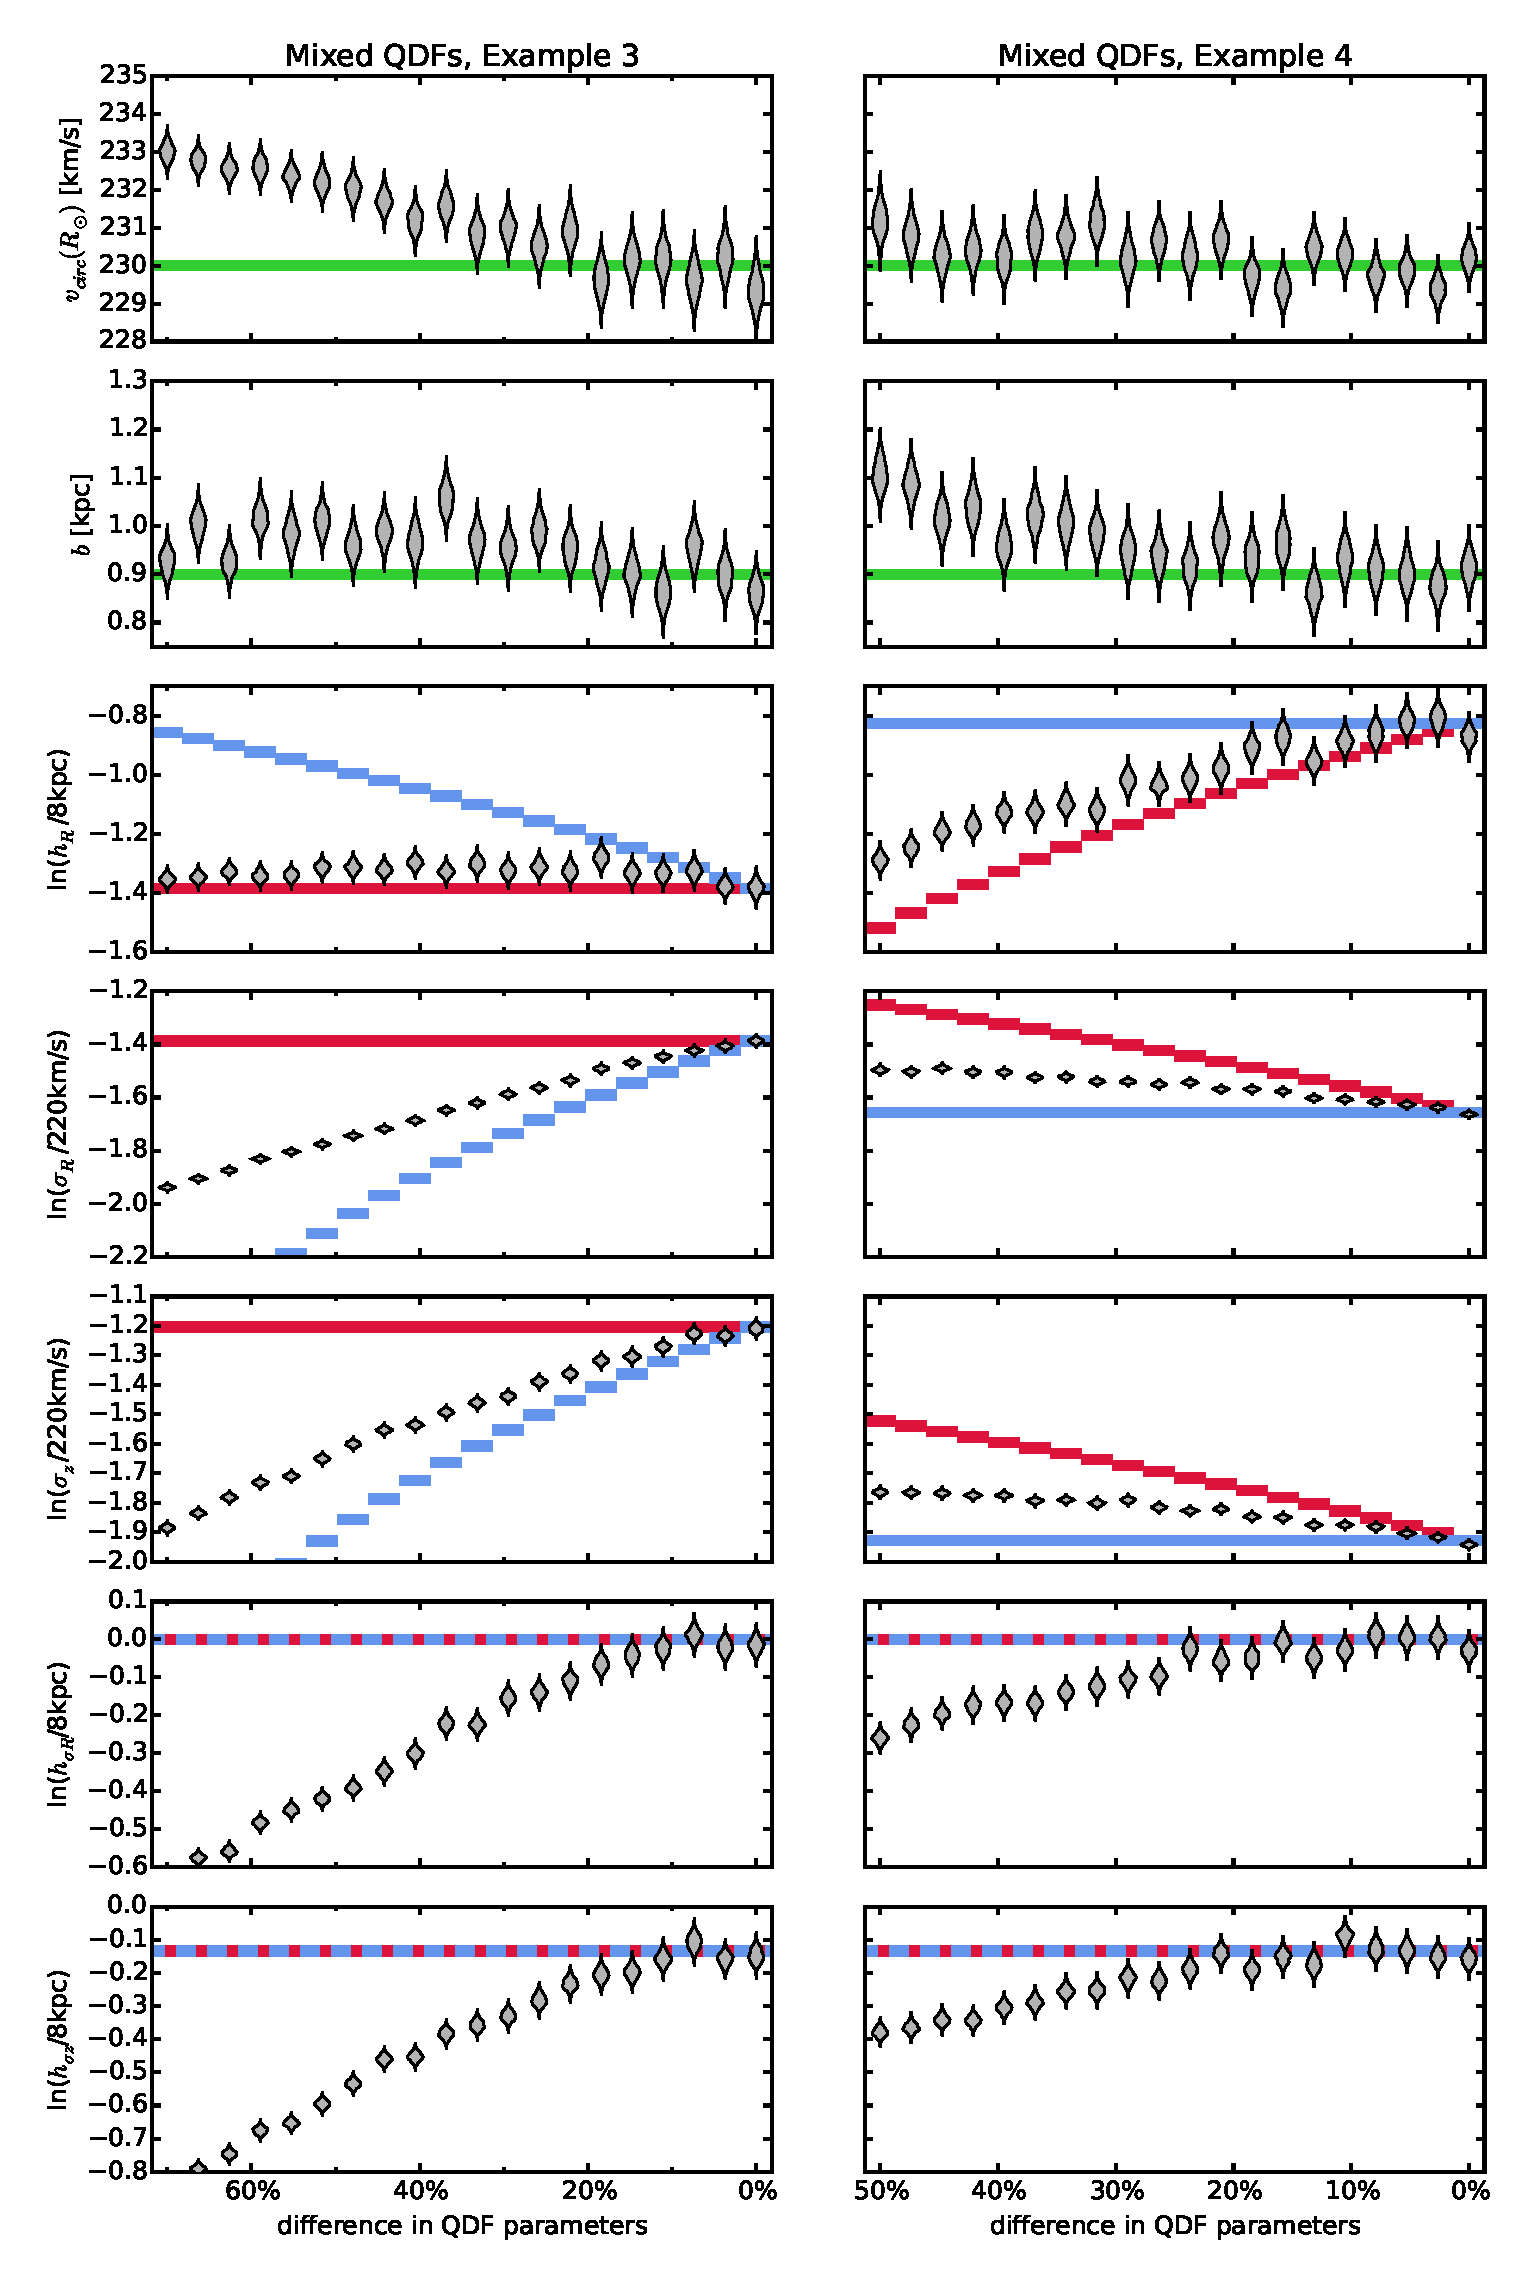
\includegraphics[width=0.8\textwidth]{figs/isoSphFlexMixDiff_violins.eps}
\caption{(Caption on next page.)}
\end{figure*}


\addtocounter{figure}{-1}
\begin{figure*} [t!]
\caption{The dependence of the parameter recovery on the difference in qDF parameters of a 50\%/50\% mixture of two stellar populations and their temperature. Half of the star in each mock data set in \emph{Example 2a} (\emph{Example 2b}) was drawn from the "hot" ("cool") qDF in Table \ref{tbl:referenceMAPs}, and the other half drawn from a "colder" ("warmer") population that has $X\%$ smaller (larger) $\sigma_R$ and $\sigma_z$ and $X\%$ larger (smaller) $h_R$. Each composite mock data set is then fitted by a single qDF and the marginalized MCMC likelihoods for the best fit parameters are shown as violins. The model parameters used for the mock data creation are given as Test \textcircled{7}, \emph{Example 2a) \& b)} in Table \ref{tbl:tests}. Some mock data sets are shown in figure \ref{fig:isoSphFlexMix_mockdata_residuals}, last two rows, where the distributions have the same colors as the corresponding best fit violins here. By mixing \MAPs with varying difference in their qDF parameters, we model the effect of bin size in the [Fe/H]-[$\alpha$/Fe] plane when sorting stars into different \MAPs: The smaller the bin size, the smaller the difference in qDF parameters of stars in the same bin. We find that the bin sizes should be chosen such that the difference in qDF parameters between neighbouring \MAPs is less than 20\%.} 
\label{fig:isoSphFlexMixDiff}
\end{figure*}

%====================================================================

%\input{docs/results_potentials_v2.01}
%%-----------------------------------------------------------------------------------------------------------------------------------------------------------------------------
%
%%-----------------------------------------------------------------------------------------------------------------------------------------------------------------------------
%%Discussion etc.
%\input{docs/discussion_and_summary_v2.01}
%\input{docs/acknowledgments_v2.01}
%%-----------------------------------------------------------------------------------------------------------------------------------------------------------------------------
%
%\begin{appendix}
%\section{Appendix}
%\input{docs/appendix_v2.01}
%\end{appendix}
%
%\input{docs/TODO_v2.01}
%
%
%
%
%
%
%
%%
%[TO DO: Check if all references are actually used in paper. ???]
%
%\begin{thebibliography}{}
%\bibitem[Batsleer \& Dejonghe(1994)]{bat94} Batsleer, P., \& Dejonghe, H. 1994, A\& A [TO DO], 287, 43
%\bibitem[Binney(2010)]{bin10} Binney, J. J. 2010, \mnras, 401, 2318
%\bibitem[Binney \& McMillan(2011)]{bin11} Binney, J. J., \& McMillan, P. 2011, \mnras, 413, 1889
%\bibitem[Binney(2011b)]{bin11b} Binney, J. 2011, Pramana, 77, 39
%\bibitem[Binney(2012)]{bin12} Binney, J. J. 2012a, \mnras, 426, 1324
%\bibitem[Binney(2012)]{bin12b} Binney, J. J. 2012b, \mnras, 426, 1328 (Princeton University Press)
%\bibitem[Binney \& Tremaine(2008)]{bin08} Binney, J. \& Tremaine, S. 2008, Galactic Dynamics: Second Edition
%\bibitem[Bissantz et al.(2004)]{bis04} Bissantz, N., Debattista, V. P., \& Gerhard, O. 2004, \apj, 601, L155
%\bibitem[Bovy \& Tremaine(2012)]{bt12} Bovy, J., \& Tremaine, S. 2012, \apj, 756, 89
%\bibitem[Bovy et al.(2012b)]{bov12b} Bovy, J., Rix, H.-W., \& Hogg, D. W. 2012b, \apj, 751, 131
%\bibitem[Bovy et al.(2012c)]{bov12c} Bovy, J., Rix, H.-W., Hogg, D. W. et al., 2012c, \apj, 755,115
%\bibitem[Bovy et al.(2012d)]{bov12d} Bovy, J., Rix, H.-W., Liu, C. et al., 2012d, \apj, 753, 148
%\bibitem[Bovy \& Rix(2013)]{bov13}  Bovy, J., \& Rix, H.-W. 2013, \apj, 779, 115
%\bibitem[Bovy(2015)]{bov15} Bovy, J. 2015, ApJS, 216, 29 [TO DO]
%\bibitem[B\"{u}denbender et al.(2015)]{bue15} B\"{u}denbender, A., van de Ven, G., \& Watkins, L. L. 2015, \mnras, 452, 956
%\bibitem[Dehnen \& Binney(1998)]{deh98} Dehnen, W., \& Binney, J. 1998, \mnras, 294, 429
%\bibitem[Dehnen(1998)]{1998AJ....115.2384D} Dehnen, W.\ 1998, \aj, 115, 
%2384 
%\bibitem[De Lorenzi et al.(2007)]{lor07} De Lorenzi F., Debattista V.P., Gerhard O., Sambhus N. 2007, \mnras, 376, 7
%\bibitem[Famaey \& Dejonghe(2003)]{2003MNRAS.340..752F} Famaey, B., \& Dejonghe, H.\ 2003, \mnras, 340, 752 
%\bibitem[Foreman-Mackey et al.(2013)]{for13} Foreman-Mackey, D., Hogg, D. W., Lang, D., \& Goodman, J. 2013, PASP [TO DO], 125, 306
%\bibitem[Gilmore \& Reid(1983)]{gil83} Gilmore, G. \& Reid, N. 1983, \mnras, 202, 1025
%\bibitem[Holmberg et al.(2009)]{2009A&A...501..941H} Holmberg, J., Nordstr{\"o}m, B., \& Andersen, J.\ 2009, \aap, 501, 941 
%\bibitem[Hunt \& Kawata(2014)]{hun14} Hunt, J. A. S., \& Kawata, D. 2014, \mnras, 443, 2112
%\bibitem[Johnston et al.(1999)]{joh99} Johnston, K. V., Zhao, H. S., Spergel, D. N., \& Hernquist, L. 1999, ASPC [TO DO], 194, 15
%\bibitem[Juri{\'c} et al.(2008)]{jur08} Juri{\'c}, M., Ivezi{\'c}, {\v Z}., Brooks, A., et al.\ 2008, \apj, 673, 864 
%\bibitem[Kawata et al.(2014)]{2014MNRAS.443.2757K} Kawata, D., Hunt, J.~A.~S., Grand, R.~J.~J., Pasetto, S., \& Cropper, M.\ 2014, \mnras, 443, 2757 
%\bibitem[Klement et al.(2008)]{2008ApJ...685..261K} Klement, R., Fuchs, B., \& Rix, H.-W.\ 2008, \apj, 685, 261 
%\bibitem[Loebman et al.(2012)]{loe12} Loebman, S. R., Ivezic, Z., Quinn, T. R. et al., 2012, \apj, 758L, 23
%\bibitem[McMillan(2011)]{mcm11} McMillan, P. 2011, \mnras, 414, 2446
%\bibitem[McMillan \& Binney(2008)]{2008MNRAS.390..429M} McMillan, P.~J., \& Binney, J.~J.\ 2008, \mnras, 390, 429 
%\bibitem[McMillan \& Binney(2012)]{2012MNRAS.419.2251M} McMillan, P.~J., \& Binney, J.\ 2012, \mnras, 419, 2251 
%\bibitem[McMillan \& Binney(2013)]{2013MNRAS.433.1411M} McMillan, P.~J., \& Binney, J.~J.\ 2013, \mnras, 433, 1411 
%\bibitem[Minchev et al.(2011)]{2011A&A...527A.147M} Minchev, I., Famaey, B., Combes, F., et al.\ 2011, \aap, 527, A147 
%\bibitem[Navarro et al.(2004)]{2004ApJ...601L..43N} Navarro, J.~F., Helmi, 
%A., \& Freeman, K.~C.\ 2004, \apjl, 601, L43 
%\bibitem[Ness et al.(2015)]{nes15} Ness, M., Hogg, D. W., Rix, H.-W. et al., 2015, \apj, 808, 16
%\bibitem[Nordstr{\"o}m et al.(2004)]{2004A&A...418..989N} Nordstr{\"o}m, B., Mayor, M., Andersen, J., et al.\ 2004, \aap, 418, 989 
%\bibitem[Perryman et al.(2001)]{2001A&A...369..339P} Perryman, M.~A.~C., de Boer, K.~S., Gilmore, G., et al.\ 2001, \aap, 369, 339 
%\bibitem[Piffl et al.(2014)]{pif14} Piffl, T., Binney, J., \& McMillan, P. J. et al., 2014, \mnras, 455, 3133
%\bibitem[Rix \& Bovy(2013)]{rix13} Rix, H.-W., \& Bovy, J. 2013, [TO DO] A\& ARv, 21, 61
%\bibitem[Ro\v{s}kar et al.(2008a)]{ros08a} Ro\v{s}kar, R., Debattista, V. P., Stinson, G. S., Quinn, T. R., Kaufmann, T., \& Wadsley, J. 2008a, \apj, 675, L65
%\bibitem[Ro\v{s}kar et al.(2008b)]{ros08b} Ro\v{s}kar, R., Debattista, V. P., Quinn, T. R., Stinson, G. S., \& Wadsley, J. 2008b, \apj, 684, L79
%\bibitem[Sackett(1997)]{sac97} Sackett, P. 1997, \apj, 483, 103
%\bibitem[Sanders \& Binney(2015)]{san15} Sanders J. L., Binney J. 2015, \mnras, 449, 3479
%\bibitem[Sch\"{o}nrich \& Binney(2008)]{sch08} Sch\"{o}nrich, R. \& Binney, J. J. 2008, \mnras, 396, 203
%\bibitem[Sellwood(2010)]{2010MNRAS.409..145S} Sellwood, J.~A.\ 2010, \mnras, 409, 145 
%\bibitem[Sellwood \& Binney(2002)]{sel02} Sellwood, J. A., \& Binney, J. J. 2002, \mnras, 336, 785
%\bibitem[Steinmetz et al.(2006)]{ste06} Steinmetz, M. et al., 2006, \aj, 132, 1645
%\bibitem[Syer \& Tremaine(1996)]{sye96} Syer D., Tremaine S. 1996, \mnras, 282, 223
%\bibitem[Ting et al.(2013)]{tin13} Ting, Y.-S., Rix, H.-W., Bovy, J., \& van de Ven, G. 2013, \mnras, 434, 652
%\bibitem[Xue et al.(2015)]{2015arXiv150606144X} Xue, X.-X., Rix, H.-W., Ma, Z., et al.\ 2015, arXiv:1506.06144 
%\bibitem[Yanny et al.(2009)]{yan09} Yanny, B., Newberg, H.-J., Johnson, J. A., et al. 2009, \aj, 137, 4377 
%\bibitem[Zhang et al.(2013)]{zha13} Zhang, L., Rix, H.-W., van de Ven, G. et al., 2013, \apj, 772, 108
%\end{thebibliography}
%
%[TO DO: Mit wie vielen J. wird Binney geschrieben?] [TO DO: Kommas nach letztem Namen oder nicht?] [TO DO: In welcher Reihenfolge soll ich sortieren?] [TO DO: Wie viele Autoren nennen, bevor et al.???]

%-----------------------------------------------------------------------------------------------------------------------------------------------------------------------------
%Long landscape tables
\clearpage
%\LongTables
\begin{landscape}
\begin{deluxetable}{llllll}
\tabletypesize{\scriptsize}
%\rotate
\tablecaption{Gravitational potentials of the reference galaxies used troughout this work and the respective ways to calculate actions in these potentials. All four potentials are axisymmetric. The potential parameters are fixed for the mock data creation at the values given in this table. In the subsequent analyses we aim to recover these potential parameters again. The parameters of "MW13-Pot" and "KKS-Pot" were found as direct fits to the "MW14-Pot". \label{tbl:referencepotentials}}
\tablewidth{0pt}
\tablehead{
\colhead{name} & \colhead{potential type} & \multicolumn{2}{c}{potential parameters $p_\Phi$} & \colhead{action calculation} & \colhead{reference for potential type}}
\startdata
"Iso-Pot" & isochrone potential   & circular velocity at the sun             & $v_\text{circ}$ = $230$ km s$^{-1}$           & \textbf{\emph{analytical and exact}} $J_r, J_\vartheta, L_z$;     & \citet{bin08} \\
          &					      & isochrone scale length                   & $b$ = $0.9$ kpc                               & use $J_r \rightarrow J_R, J_\vartheta \rightarrow J_z $  &               \\
          &                       &                                          &                                               & in Eq. (\ref{eq:df_general})                                             &               \\
\tableline
"KKS-Pot" & 2-component                  & circular velocity at the sun             & $v_\text{circ}$ = $230$ km s$^{-1}$           & \textbf{\emph{exact}} $J_R, J_z, L_z$       & \citet{bat94} \\
          & Kuzmin-Kutuzov-              & focal distance of coordinate system\tablenotemark{a}       & $\Delta = 0.3$              & using "St\"{a}ckel Fudge"                   &               \\                                                                
          & St\"{a}ckel potential        & axis ratio of the coordinate surfaces\tablenotemark{a} ... &                             & \citep{bin12}                               &               \\
          & \hspace{0.3cm} (disk + halo) & \hspace{0.3cm} ...of the disk component   & $\left(\frac{a}{c}\right)_\text{Disk}$ = 20  & and interpolation                           &               \\
          &                              & \hspace{0.3cm} ...of the halo component   & $\left(\frac{a}{c}\right)_\text{Halo}$ = 1.07& on action grid\tablenotemark{b}                              &               \\
          & (analytic potential)         & relative contribution of the disk mass    &                                              & \citep{bov15}                               &               \\
          &                              & \hspace{0.3cm} to the total mass          & $k = 0.28$                                   &                                             &               \\  
\tableline
"MW13-Pot" & MW-like potential with        & circular velocity at the sun             & $v_\text{circ}$ = $230$ km s$^{-1}$           & \textbf{\emph{approximate}} $J_R, J_z, L_z$ & \citet{bov13} \\          
           & Hernquist bulge,              & stellar disk scale length                & $R_d = 3$ kpc                                 & using "St\"{a}ckel Fudge"          &               \\
           & 2 exponential disks           & stellar disk scale height                & $z_h = 0.4$ kpc                               & \citep{bin12}                      &               \\
           & \hspace{0.3cm} (stars + gas), & relative halo contribution to $v_\text{circ}^2(R_\odot)$ & $f_h = 0.5$                   & and interpolation                  &               \\
           & spherical power-law halo      & "flatness" of rotation curve & $\frac{\diff \ln(v_\text{circ}(R_\odot))}{ \diff \ln(R)}$ = 0  & on action grid\tablenotemark{a}                &               \\
           & (interpolated potential)      &                                          &                                               & \citep{bov15}                      &               \\
\tableline
"MW14-Pot" & MW-like potential with        &  -                                       & -                                             & \textbf{\emph{approximate}} $J_R, J_z, L_z$ & \citet{bov15} \\
           & cut-off power-law bulge,       &                                          &                                               & (see "MW13-Pot")                   &               \\
           & Miyamoto-Nagai stellar disk,  &                                          &                                               &                                    &               \\
           & NFW halo                      &                                          &                                               &                                    &               \\
\enddata
\tablenotetext{a}{The coordinate system of each of the two St\"{a}ckel-potential components is $\frac{R^2}{\tau_{i,p}+\alpha_p} + \frac{z^2}{\tau_{i,p}+\gamma_p}=1$ with $p \in \{\text{Disk},\text{/Halo}\}$ and $\tau_{i,p} \in \{\lambda_p,\nu_p\}$. Both components have the same focal distance $\Delta = \sqrt{\gamma_p-\alpha_p}$, to make sure that the superposition of the two components itself is still a St\"{a}ckel potential. The axis ratio of the coordinate surfaces $\left(\frac{a}{c}\right)_p := \sqrt{\frac{\alpha_p}{\gamma_p}}$ describes the flattness of the corresponding St\"{a}ckel component.}
\tablenotetext{b}{We use a finely spaced action interpolation grid with $R_\text{max}=10$ [TO DO: What's that??? units???] and 50 grid points in $E$ and $\psi$ [TO DO: Find out what's that???], and 60 grid points in $L_z$. [TO DO: more details?]}
\end{deluxetable}

\begin{deluxetable}{lccccc}
\tabletypesize{\scriptsize}
%\rotate
\tablecaption{Reference distribution function parameters for the qDF in eq. (\ref{eq:df_general})-(\ref{eq:sigmazRg}). These qDFs describe the phase-space distribution of stellar \MAPs for which mock data is created and analysed throughout this work for testing purposes. The parameters of the "cooler" \& "colder"  ("hotter" \& "warmer") \MAPs were chosen such, that the they have the same $\sigma_R/\sigma_z$ ratio as the "hot" ("cool") \MAP. The "colder" and "warmer" \MAPs have a free parameter $X$ that governs how much colder/warmer they are then the reference "hot" and "cool" qDFs. Hotter populations have shorter tracer scale lengths \citep{bov12d} and the velocity dispersion scale lengths were fixed according to \citet{bov12c}. \label{tbl:referenceMAPs}}
\tablewidth{0pt}
\tablehead{
\colhead{name of \MAP} & \multicolumn{5}{c}{qDF parameters $p_\text{DF}$}\\
                       & \colhead{$h_R$ [kpc]} & \colhead{$\sigma_R$ [km s$^{-1}$]} & \colhead{$\sigma_z$ [km s$^{-1}$]} & \colhead{$h_{\sigma_R}$ [kpc]} & \colhead{$h_{\sigma_z}$ [kpc]}}
\startdata
"hot"    & 2   & 55 & 66 & 8 & 7\\
"cool"   & 3.5 & 42 & 32 & 8 & 7\\
\tableline
"cooler" & 2  +50\% & 55-50\% & 66-50\% & 8 & 7 \\
"hotter" & 3.5-50\% & 42+50\% & 32+50\% & 8 & 7\\
\tableline
"colder" & 2  +X\% & 55-X\% & 66-X\% & 8 & 7 \\
"warmer" & 3.5-X\% & 42+X\% & 32+X\% & 8 & 7\\
\enddata
\end{deluxetable}

\begin{deluxetable}{lllll}%{p{0.1\textwidth}p{0.1\textwidth}p{0.25\textwidth}p{0.25\textwidth}p{0.05\textwidth}}
\tabletypesize{\scriptsize}
%\rotate
\tablecaption{Summary of test suites in this work: The first column indicates the test suite, the second column the potential, DF and selection function model etc. used for the mock data creation, the third model the corresponding model assumed in the analysis, and the last column lists the figures belonging to the test suite. Parameters that are not left free in the analyis, are always fixed to their true value. Unless otherwise stated we calculate the likelihood by the nested-grid and MCMC approach outlined in \S\ref{sec:fitting} and use $N_\text{spatial} = 16$, $N_\text{velocity} = 24$, $N_\text{sigma} = 5$ as numerical accuracy for the likelihood normalisation in Eq. (\ref{eq:prob}) and (\ref{eq:tracerdensity}). [TO DO: Change encircled numbers to proper order. Make sure the plot references are the right ones.] \label{tbl:tests}}
\tablewidth{0pt}
\tablehead{
\colhead{Test} & & \colhead{Model for Mock Data}  & \colhead{Model in Analysis} & \colhead{Figures}}
\startdata
\textcircled{1}         & \emph{Potential:}     & "KKS-Pot" & - & Mock data: \\
Influence of            & \emph{\MAP:}          & 2 \MAPs "hot" or "cold" qDF   &   & Fig. \ref{fig:mockdatadistr}\\
survey volume on        & \emph{Survey volume:} & a) $R \in [4,12]$ kpc,$z \in [-4,4]$ kpc, $\phi \in [-20^\circ,20^\circ]$. &  & \\
mock data distribution, &                       & b) $R \in [6,10]$ kpc,$z \in [1,5]$ kpc, $\phi \in [-20^\circ,20^\circ]$.&  & \\
also in action space	& \emph{\# stars per data set:} & 20,000 &  & \\
						& \emph{\# data sets:}   & 4 (= $2\times 2$ models) & & \\

\tableline
\textcircled{9}         & \emph{Potential:}     & "Iso-Pot", "MW13-Pot" \& "KKS-Pot" & - & Convergence\\
Numerical accuracy      & \emph{\MAP:}          & "hot" qDF                          &   & of normalisation:\\
in calculation          & \emph{Survey volume:} & sphere around sun, $r_\text{max} = 0.2, 1, 2, 3$ or $4$ kpc &   & Fig. \ref{fig:norm_accuracy}\\
of the likelihood       & \emph{Numerical accuracy:} & $N_\text{spatial}\in[5,20]$, $N_\text{velocity}\in[6,40]$, $N_\text{sigma}\in[3.5,7]$& & \\
normalisation           &                       & & & \\
										   
\tableline
\textcircled{10}        & \emph{Potential:}     & "Iso-Pot" & "Iso-Pot", all parameters free & Fig. \ref{fig:triangleplot}\\
\pdf is a               & \emph{\MAP:}          & "hot" qDF & qDF, all parameters free & \\
multivariate            & \emph{Survey Volume:} & sphere around sun, $r_\text{max} = 2$ kpc & (fixed \& known) & \\
Gaussian                & \emph{\# stars per data set:} & 20,000 & & \\
for large data sets.	& \emph{\# data sets:}   & 5 (only one is shown) & & \\
                        & \emph{Numerical accuracy:} & & $N_\text{velocity} = 20$ and $N_\text{sigma} = 4$ & \\

\tableline
\textcircled{2}			& \emph{Potential:}     & "Iso-Pot" & "Iso-Pot", free parameter: $b$ & Fig. \ref{fig:sqrtN}\\
Width of the			& \emph{\MAP:}          & "hot" qDF & "hot" qDF, free parameters: & \\
likelihood scales       &                       &           & $\ln\left(\frac{h_R}{8\text{kpc}}\right),\ln\left(\frac{\sigma_{R}}{230 \text{km s}^{-1}}\right),\ln\left(\frac{h_{\sigma,R}}{8\text{kpc}}\right)$ & \\
with number of stars    & \emph{Survey volume:} & sphere around sun, $r_\text{max} = 3$ kpc   & (fixed \& known) & \\
by $\propto 1/\sqrt{N}$.& \emph{\# stars per data set:} & between 100 and 40,000 &  & \\ 
                        & \emph{\# data sets:}  & 132 & & \\                                       
                        & \emph{Analysis method:} & & likelihood on grid & \\
                        & \emph{Numerical accuracy:} & & $N_\text{velocity} = 20$ and $N_\text{sigma} = 4$ (for speed) & \\

\tableline
\textcircled{3}         & \emph{Potential:}     & 2 "Iso-Pot" with & "Iso-Pot", free parameter: $b$ & Fig. \ref{fig:centrallimittheorem}\\
Parameter estimates     &                       & $b=0.8$ kpc or $b=1.5$ kpc & \\
are unbiased.           & \emph{\MAP:}          & 2 \MAPs, "hot" or "cool" qDF  & "hot"/"cool" qDF, free parameters: & \\
                        &                       &                          & $\ln\left(\frac{h_R}{8\text{kpc}}\right),\ln\left(\frac{\sigma_{R}}{230 \text{km s}^{-1}}\right),\ln\left(\frac{h_{\sigma,R}}{8\text{kpc}}\right)$ & \\
                        & \emph{Survey volume:} & 5 spheres around sun, $r_\text{max} = 0.2, 1, 2, 3$ or $4$ kpc & (fixed \& known) & \\
                        & \emph{\# stars per data set:} & 20,000 & & \\
                        & \emph{\# data sets:}  & 640 (= $2\times2\times5$ models $\times 32$ realisations) & & \\
                        & \emph{Analysis method:} & & likelihood on grid & \\
                        & \emph{Numerical accuracy:} & & $N_\text{velocity} = 20$ and $N_\text{sigma} = 4$ (for speed) & \\

\tableline
\textcircled{4} 		& \emph{Potential:} 	& i) "Iso-Pot", ii) "MW13-Pot" or iii) "KKS-Pot" 	& i) "Iso-Pot", all parameters free & Fig. \ref{fig:wedFlexVol_bias_vs_SE} \\
Influence of 			& 						& 													& ii) "MW13-Pot", $R_d$ and $f_h$ free & \\
position \& shape 		& 						& 													& iii) "KKS-Pot", all free except $v_\text{circ}(R_\odot)$ & \\
of survey volume 		& \emph{\MAP:}			& "hot" qDF 										& i) \& iii) qDF, all parameters free & \\
on parameter recovery 	& 						& 													& ii) qDF, only $h_R$, $\sigma_{z,0}$ and $h_{\sigma_R}$ free& \\
						& \emph{Survey volume:}	& 4 different wedges, see Fig. \ref{fig:wedFlexVol_bias_vs_SE}, upper right panel & (fixed \& known) & \\
						& \emph{\# of stars per data set:} & 20,000 & & \\
						& \emph{\# data sets:}	& 48 (= $4\times3$ models $\times 4$ realisations) & & \\
						& \emph{Analysis method:} & & i) \& ii) MCMC, iii) likelihood on grid & \\
						& \emph{Action calculation:} & ii) \& iii) low accuracy & (same as mock data creation) & \\
						&						& "St\"{a}ckel Fudge" grid \citep{bov15} for speed && \\
						&						& (\# grid points: 25 in each $E$ and $\psi$, && \\
						&						& 30 in $L_z$, $R_\text{max}=5$  & & \\
						&						& [TO DO: What is psi and Rmax (units)?]) & & \\
\tableline
\textcircled{5}         & \emph{Potential:}     & "Iso-Pot" & "Iso-Pot", all parameters free & Illustration \& mock data: \\
Influence of            & \emph{\MAP:}          & 2 \MAPs, a) "hot" or b) "cool" qDF & qDF, all parameters free &  Fig. \ref{fig:isoSphFlexIncompR_mockdata} \& \ref{fig:isoSphFlexIncompZ_mockdata} \\
wrong assumptions       & \emph{Survey volume:} & sphere around sun, $r_\text{max} = 3$ kpc & (fixed \& known) & Analysis results: \\
about the data set      & \emph{Completeness:}  & \emph{Example 1:} radial incompleteness,  & data set complete, & Fig. \ref{fig:isoSphFlexIncompR_violins} \& \ref{fig:isoSphFlexIncompZ_violins} \\
(in-)completeness       &                       & completeness$(r) = 1-\epsilon_r \frac{r}{r_\text{max}}$, twenty $\epsilon_r \in [0,0.7]$ & completeness$(r)$ = 1, $\epsilon_r=0$& Analysis results:\\
on parameter recovery   &                       & $r \equiv$ distance from sun, & & when not using $v_T$ data: \\
                        &                       & \emph{Example 2:} planar incompleteness,  & data set complete, & Fig. \ref{fig:isoSphFlexIncomp_marginal_violins}\\
                        &                       & completeness$(z) = 1-\epsilon_z \frac{|z|}{r_\text{max}}$, $\epsilon_r \in [0,0.7]$, & completeness$(r)$ = 1, twenty $\epsilon_z=0$& \\
                        &                       & $z \equiv$ distance from Gal. plane. & & \\
                        & \emph{\# stars per data set:} & 20,000 & & \\
                        & \emph{\# data sets:}  & 40 (= $2 \times 2 \times 20$) & & \\
\tableline
\textcircled{6} 		& \emph{Potential:} 	& "Iso-Pot" & "Iso-Pot, all parameters free" & Fig. \ref{fig:isoSphFlexErrConv_MC_vs_error}\\
Numerical convergence 	& \emph{\MAP:}			& "hot" qDF & qDF, all parameters free & \\
of deconvolution		& \emph{Survey Volume:}	& sphere around sun, $r_\text{max} = 3$ kpc & (fixed \& known) & \\
with measurement		& \emph{Errors:}		& $\delta(R.A.)=\delta(DEC.)=\delta(m-M)=0$	& Deconvolution with	& \\
errors					&						& $\delta(v_\text{los}) = 2$ km/s	& perfectly known errors & \\
						&						& $\delta(\mu_\text{R.A.})= \delta(\mu_\text{DEC.}) =$ 2,3,4 or 5 mas/yr & & \\
						& \emph{Numerical Accuracy:} & & convolution using MC integration & \\
						&							 & & with between 25 and 1200 MC samples & \\
						& \emph{\# stars per data set:} & 10,000 & & \\
						& \emph{\# data sets:}	& 16 (= $4 \times 4$ realisations) & & \\
\tableline
\textcircled{12}
Testing the 			& \emph{Potential:} 	& "Iso-Pot" & "Iso-Pot, all parameters free" & Fig. \ref{fig:isoSphFlexErrConv_bias_vs_SE}\\
deconvolution 			& \emph{\MAP:}			& "hot" qDF & qDF, all parameters free & \\
with measurement		& \emph{Survey Volume:}	& sphere around sun, $r_\text{max} = 3$ kpc & (fixed \& known) & \\
errors with \& without  & \emph{Errors:}		& $\delta(R.A.)=\delta(DEC.)=0$	& Deconvolution with errors,	& \\
distance errors			&						& $\delta(v_\text{los}) = 2$ km/s & ignoring distance errors in position (see \S [TO DO: CHECK???]) & \\
						&						& $\delta(\mu_\text{R.A.})= \delta(\mu_\text{DEC.}) =$ 1, 2,3,4 or 5 mas/yr & \\
						&						& a) $\delta(m-M) = 0$, b) $\delta(m-M) \neq 0$ (see Fig. \ref{fig:isoSphFlexErrConv_bias_vs_SE}) & \\
						& \emph{Numerical Accuracy:} & & 800 or 1200 MC samples & \\
						& \emph{\# stars per data set:} & 10,000 & & \\
						& \emph{\# data sets:}	& 40 (= $2 \times 5 \times 4$ realisations) & & \\
\tableline
\textcircled{11}	& \emph{Potential:}		& "Iso-Pot" & "Iso-Pot", all parameters free & Fig. \ref{fig:isoSphFlexErrSyst}\\
Underestimation 	& \emph{\MAP:}			& "hot" or "cool" qDF & qDF, all parameters free & \\
of proper motion 	& \emph{Survey volume:}	& sphere around sun, $r_\text{max} = 3$ kpc [TO DO: CHECK]& (fixed \& known) & \\
errors 			 	& \emph{Errors:}		& only proper motion errors & Deconvolution with proper motion errors & \\
					&						& 1, 2 or 3 mas/yr & 10\% or 50\% underestimated & \\
					& \emph{\# stars per data set:} & 10,000 & & \\
					& \emph{\# data sets:}	& 24 (= $2 \times 2 \times 3 \times 3$ realisations ) & & \\
\tableline
\textcircled{7}         & \emph{Potential:} & "Iso-Pot" & "Iso-Pot", all parameters free & mock data:\\
Deviations in the       & \emph{\MAP:}      & mix of two qDFs & single qDF, all parameters free & Fig. \ref{fig:isoSphFlexMix_mockdata_residuals}\\
assumed DF              &                   & \emph{Example 1:} with fixed qDF parameters,  & & Analysis results:\\
from the                &                   & but 20 different mixing rates: & & \ref{fig:isoSphFlexMixCont} \& Fig. \ref{fig:isoSphFlexMixDiff}\\
star's true DF          &                   & a) "hot" \& "cooler" qDF or b) "cool" \& "hotter" qDF & & \\
                        &                   & \emph{Example 2:} 20 fixed 50/50 mixtures,  & & \\
                        &                   & with varying qDF parameters (by $X\%$): & & \\
                        &                   & a) "hot" \& "colder" qDF or b) "cool" \& "warmer" qDF & & \\
                        & \emph{Survey volume:}& sphere around sun, $r_\text{max}=2$ kpc & (fixed \& known) & \\
                        & \emph{\# stars per data set:} & 20,000 & & \\
                        & \emph{\# data sets:}  & 40 (= $2 \times 2 \times 20$) & & \\
                        \tableline
\textcircled{8}			&  \emph{Potential:} & "MW14-Pot" & "KKS-Pot", all parameters free, & potential contours: \\
Deviations of the		&                    &            & only $v_\text{circ}(R_\odot)=230 \text{km s}^{-1}$ fixed & Fig. \ref{fig:MW14vsKKS2SphFlex} \\
assumed potential model	& \emph{\MAP:}       & "hot" or "cool" qDF & qDF, all parameters free & qDF recovery: \\
from the star's			& \emph{Survey volume:} & sphere around sun, $r_\text{max} = 4$ kpc & (fixed \& known) & Fig. \ref{fig:MW14vsKKS2SphFlex_violins}\\
true potential			& \emph{\# stars per data set:} & 20,000 & & \\
						& \emph{\# data sets:} & 2 & & \\
\enddata
\end{deluxetable}

[TO DO: Make alpha and delta to R.A. and DEC. everywhere.???]

\clearpage
\end{landscape}

%-----------------------------------------------------------------------------------------------------------------------------------------------------------------------------

\end{document}

